\chapter{Methodology}\label{chap:methodology}
\section{Introduction}
In this chapter, the procedure for tapping the signal from the proprietary controller and PMBLDC motor and then building a performance measurement system based on the identified signal will be listed. Furthermore, the process of developing the mathematical model and the simulation of electric vehicle on Sepang North Track will be described so that the optimal mileage strategy could be identified.

The terminology of this project is to hack and get the signal from a proprietary contoller and a PMBLDC nub motor, then a performance measurement system is built upon the signal obtained and then simulation is used for building optimal mileage strategy.

\section{Signal Identification}
The drive train of the electric vehicle that will be used for participation in Shell Eco-Marathon consists of a single hub motor with no transmission. The hub motor is a PMBLDC motor, hence a controller is needed for controlling the speed as well as running the hub motor. The controller has two parts which is the controller circuit that is responsible for signal handling and a power unit which receives the signal from the signal handling unit and create the phase current for running the PMBLDC.

The signal unit of the controller takes input signal from the throttle, the key and also the hall effect sensors signal from the PMBLDC motor before it can do the calculation and output the signal to the power unit. Apart from that, the signal unit of the controller powers the speedometer and delivers the signal (for example:  speed, battery voltage, vehicle mileage covered and the state of charge (SOC) of the battery ) for displaying at the speedometer.

Since the speedometer acts solely as a display unit, it does not have signal outputs or data logging capability. Logging the data manually by reading and recording the speed, voltage and SOC when the vehicle is running is appropriate because the electric vehilce is a single seater vehicle and it's impossible for the driver to drive and record the data simultaneously. 

Therefore, the signals need to be tapped from the signal unit of the controller in order to build a system that is able to measure, display and log the data needed. Tapping all the signals is redundant because some reading is primary (for example the voltage) whereas some readings are derived from the primary signal (for instance, the SOC of the battery is based on the voltage). Hence, identification of the primary signals should be adequate.

There are a few signal that need to be tapped from the controller and the PMBLDC motor such as:

\begin{itemize}
	\item{Speed from the controller}
	\item{Voltage from the controller}
	\item{Hall effect sensors signal from the PMBLDC motor}
\end{itemize}

Before the signal can be tapped and identified, the nature of the signal should be known. The voltage signal is an analog signal which is delivered directly from the battery through the controller. On the other hand, the speed signal should be an analog signal as well since the controller takes the signal of hall effect sensors, calculate the interval between each state change and multiply with the number of poles and the wheel diameter and get the speed of the vehicle as shown in equation \ref{eq:wheelSpeedHall}, where \textit{V} is the wheel speed, \textit{D} is the wheel diameter, \textit{N} is the number of poles of the PMBLDC motor and \textit{t} is the interval between changing state of the hall effect sensor.

\begin{equation}
	\label{eq:wheelSpeedHall}
	\text{\myequations{Wheel speed for direct drive based on hall effect sensor signal, wheel diameter and PMBLDC number of poles}}
	V = \frac{\pi D}{2Nt}
\end{equation}

Figure \ref{im:hall_signal} shows the hall effect signals which is a square wave. The hall effect sensor is a sensor where the output voltage from the sensor will change from minimum to maximum or vise versa depending on the circuit configuration. Since the sensor circuit is set in a way that it ampliefies the signal and output high/low when the magnetic field of the rotor is detected as shown in figure \ref{im:hall_circuit}, the signal output of the hall effect sensors is a square wave.

\begin{figure} [htb]
	\centering
	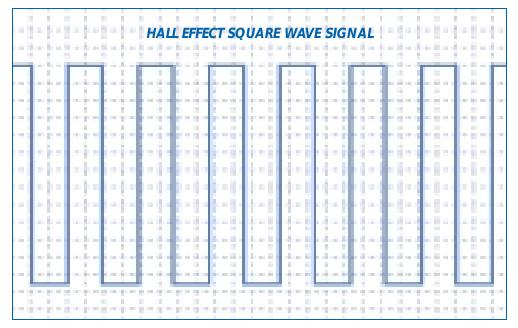
\includegraphics[width=3in]{images/hall_effect_signals.jpg}
	\caption{Hall effect sensor square wave signal \citep{counterpoint31}}
	\label{im:hall_signal}
\end{figure}

\begin{figure} [htb]
	\centering
	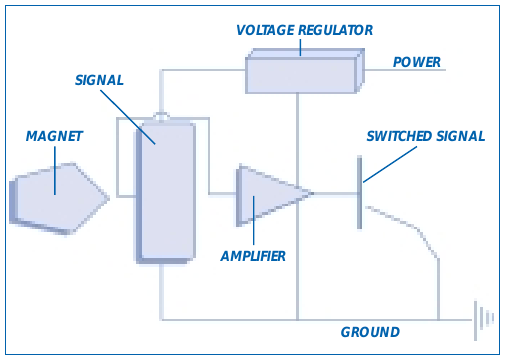
\includegraphics[width=3in]{images/hall_sensor_circuit.png}
	\caption{Circuit of hall effect sensor \citep{counterpoint31}}
	\label{im:hall_circuit}
\end{figure}

There are 16 ports for signal and power from the controller to the speedometer as shown in figure \textbf{...}. The method for detecting the signal is trial and error and elimination. The ground port is found using the digital multimeter where the two probes of the digital multimeter is plug in to any 2 ports. The port where it is constantly lower voltage than the other 15 ports is the ground port.

After the ground port is found, the procedure above is repeated by testing the 15 ports by taking the ground port as reference. The voltage reading for those 15 ports is measured and recorded when the system is idle and when the motor is running. The ports for the following signal should be found:

\begin{itemize}
	\item{Speed where the reading changes when the motor is rotating and static}
	\item{Battery voltage which it is at ~50+V when the motor is idle and drops ~2V when the motor is running}
	\item{A constant voltage ~12V for powering the speedometer}
\end{itemize}

The hall effect sensor terminal is a 8 ports input/output as shown in figure \textbf{...}.. Again, the method for detecting the signal is trial and error with step by step elimination that is similar to the method used for identifying the speed signal at the controller circuit. The hall effect sensor circuit has the same circuit that is shown in figure \ref{im:hall_circuit} except that it has 3 sensors signal output instead of 1 output. 

The hall effect sensor tapping is started with the identification of the voltage input to the hall effect sensors circuit. The voltage input to the circuit is 12V, hence, using the same method as speed signal detection, the digital multimeter's probe is plug into the any 2 ports of the 8 I/O ports within the terminal and detect the port with 12V reading.

After the voltage input ports is identified, the 3 hall effect sensors output signal is tapped by again plugging in the ground probe to the ground input port and the other positive probe to any 1 of the 6 remaining ports. The wheel is rotated manually over a revolution and the ports that produce ups and downs voltage signal would be the hall effect sensors output port.

After the hall effect sensors output port has been identified, the probes of the multimeter is plugged into the first hall effect sensor output port and the ground port. The wheel is rotated by hand over a precise 1 revolution and the number of square wave over a wheel revolution is measured and the signal output at each 10 \textdegree is measured and recorded. The same procedures apply to the other 2 hall effect sensors output ports. A graph of hall effect sensors signals versus the angle is then plot.

\section{Measurement System}
After the primary signal (speed and voltage) is identified, a measurement that has the ability to measure, display and log the parameters need to be built. The purpose of building the measurement system is to

\begin{itemize}
	\item{Measure and log the power consumption of the electric vehicle so that the mileage of the vehicle can be known.}
	\item{Measure and log the power consumtion at each vehicle on-road speed.}
	\item{Building a speed and power consumption display for the electric vehicle.}
\end{itemize}

For measuring the power input, based on equation \ref{eq:powerInput}, the input voltage and input current need to be measured. Apart from measuring the power input to the electric vehicle, the data output from the measurement system can also be used to calculate the instantaneous deceleration of the vehicle when it's cruising, when it's braking with regenerative braking and when it's braking with regenerative and mechanical braking.

\begin{equation}
	\label{eq:powerInput}
	\text{\myequations{Power Input}}
	P_{input} = V_{input}I_{input}
\end{equation}

The measurement system uses a circuit with microcontroller, crystal and I/O pins, which is the Arduino Mega 2560 board for processing the signal from the controller circuit, calculate the real value based on the signal, log the data into a SD card through the ITDB02 shield and display the speed and power consumption value through the ITDB02-3.2(WC) LCD screen.

Since the microcontroller board can only accept I/O less than 5V and more than 0V but the battery voltage is in the range of 48V - 60V and the speed signal from the controller is negative voltage, hence an intermediate circuit has to be built so that the signal can be read by the microcontroller.

For the voltage measurement circuit, a voltage divider is built for measuring the voltage of the battery. The voltage divider is a 2 resistor circuit that has same or different value of resistance for each of the resistor as shown in figure \ref{im:voltageDivider} The voltage output, \textit{$V_{out}$} can be calculated using equation \ref{eq:voltageDivider} where \textit{R1} is the resistance for the first resistor, \textit{R2} is the resistance of the second resistor and \textit{$V_{in}$} is the voltage that need to be measured.

\begin{figure}[htb]
	\centering
	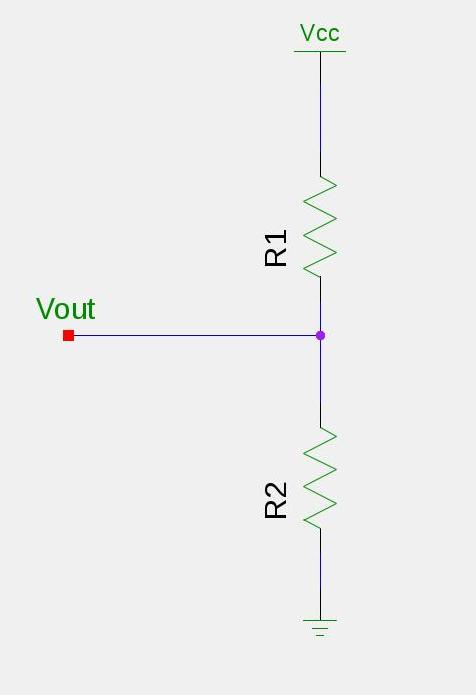
\includegraphics[width=3in]{images/voltage_divider.jpg}
	\caption{Voltage Divider}
	\label{im:voltageDivider}
\end{figure}

\begin{equation}
	\label{eq:voltageDivider}
	\text{\myequations{Voltage Divider}}
	V_{out} = \frac{V_{in}R2}{R1+R2}
\end{equation}

For measuring the speed, the same method which is the voltage divider is used with a little modification which replaces the \textit{$V_{in}$} to +5V and the ground to \textit{$V_{in}$} as shown in figure \ref{im:voltageDividerInverse} The \textit{$V_{out}$} for the modified voltage divider circuit could be calculated using equation \ref{eq:voltageDividerInverse}

\begin{figure}[htb]
	\centering
	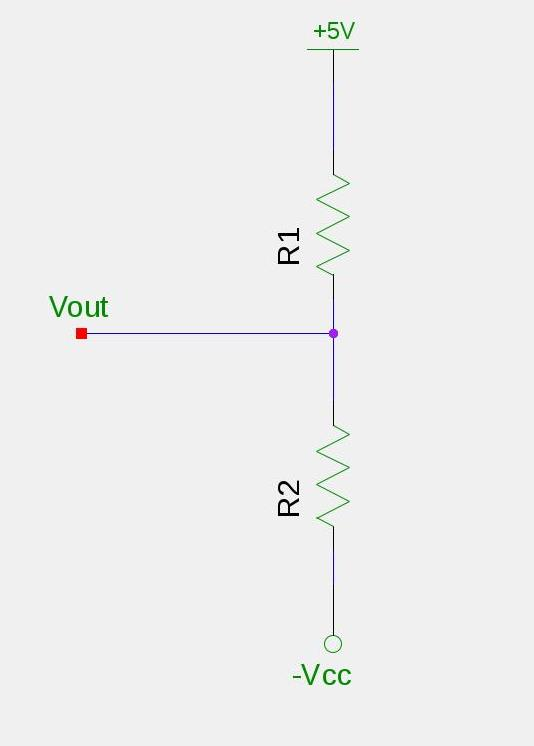
\includegraphics[width=3in]{images/voltage_divider_negative.jpg}
	\caption{Voltage Divider for negative voltage}
	\label{im:voltageDividerInverse}
\end{figure}

\begin{equation}
	\label{eq:voltageDividerInverse}
	\text{\myequations{Voltage Divider for negative voltage}}
	V_{out} = \frac{(5-V_{in})(R2)}{R1+R2} + V_{in}
\end{equation}

The resistance is selected based on the value of the negative voltage. For example, if the negative voltage is -5V, 1k\ohm \ resistor can be selected for both \textit{R1} and \textit{R2} which yields:

\centerline{$V_{out} = \frac{(5+5)(1000)}{1000+1000} - 5$}
\centerline{$V_{out} = 0V$}


If the \textit{$V_{in}$} is 0V, \textit{$V_{out}$} will be:

\centerline{$V_{out} = \frac{(5+0)(1000)}{1000+1000} - 0$}
\centerline{$V_{out} = 2.5V$}

Therefore, using a voltage divider, a negative voltage can be converted to positive voltage with minimum half of the original resolution.

The third parameter that need to be included in the measurement system is the input current. The input current is needed for calculating the input power to the electric vehicle and thus the overall vehicle mileage can be calculated. Since the rules of Shell Eco-Marathon restricted the nominal current input to the electric vehilce to be 60A and the peak current must be less than 150A, therefore a 200A current sensor is used.

The current sensor used in detecting the input current is the ALLEGRO MICROSYSTEMS ACS758ECB-200B-PFF-T which is a 200A current sensor with 5 terminals and analog voltage output signal as shown in figure \textbf{....} In order for the microcontroller to measure the current, a current measuring circuit with the current sensor is built. The schematic of the current sensor circuit is shown in figure \textbf{....}

After the prototype circuit of the current measuring circuit, the voltage measurement circuit and the speed voltage divider circuit is built, the 3 circuits is integrated into a single circuit and the microcontroller is program in a way that it can read, log and display the speed of the vehicle, the instantaneous current and voltage and the mileage covered every 100ms interval.

\section{Vehicle Simulation}
